\chapter{Bildverarbeitung}
\section{Boxfilter}
Boxfilter
Faltung
$$ \widetilde{I}(i, j)=I \ast f =  \sum_{\alpha=-m}^m \sum_{\beta=-n}^n I(i-\alpha, j-\beta) \cdot f(\alpha, \beta)$$
Relevant: 
$$ \sum_{\alpha=-m}^m \sum_{\beta=-n}^n f(\alpha, \beta) \stackrel{!}{=} 1 $$
Boxfilter - Mittelwertfilter
$$ f=\frac{1}{9} \begin{bmatrix} 1&1&1 \\ 1&1&1 \\ 1&1&1 \end{bmatrix}$$
$$ \widetilde{I}(i, j)=\frac{1}{9} \sum_{\alpha=-1}^1 \sum_{\beta=-1}^1 I(i-\alpha, j-\beta) $$
Veranschaulicht wird dieses Vorgehen in \ref{fig:boxfilter}. Im linken Abschnitt ist das Originalbild mit einem gr\"o\ss{}eren Objekt und einigen St\"orpixeln zu sehen. Im rechten Abschnitt ist die gefilterte Version zu sehen: Die einzelnen St\"orpixel im oberen Abschnitt des Bildes sind deutlich abgeschw\"acht. Die Grenzen des Objektes in der rechten, unteren Ecke sind jedoch ebenso verschwommen. Bei mehrfacher Anwendung eines Mittelwertfilters konvergieren alle Pixelwerte gegen den Mittelwert der Pixel des gesamten Bildes. Der Mittelwertfilter ist somit ein Tiefpassfilter und sorgt anschaulich daf\"ur, dass Bilder verschwimmen.
\begin{figure}
 \centering
 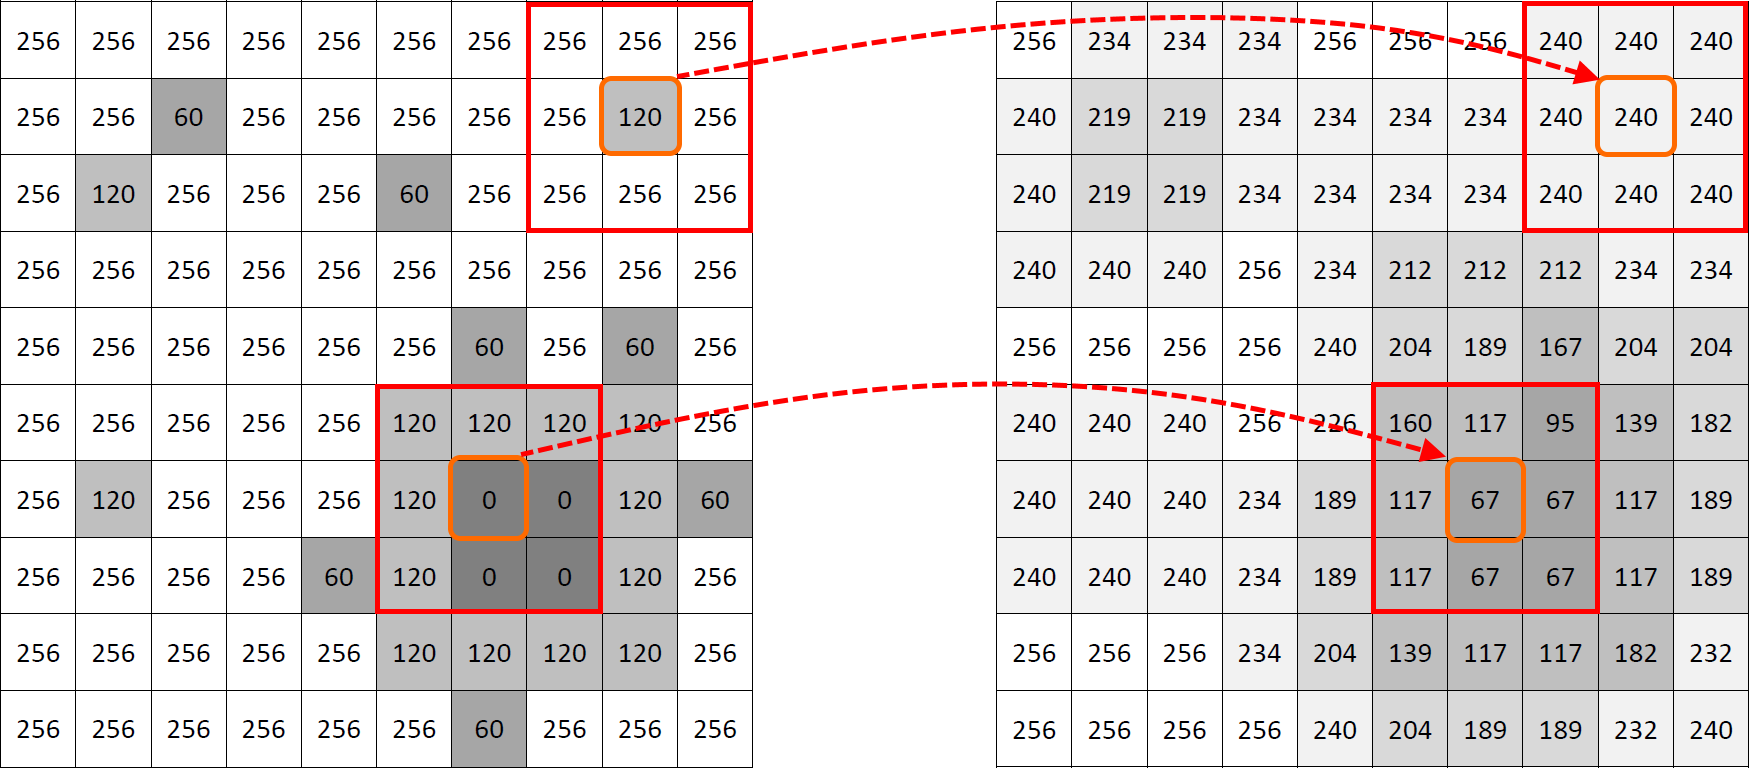
\includegraphics[width=1\textwidth]{media/filter/boxfilter_combined.png}
 \caption{Beispiel für 3x3 Boxfilter}
 \label{fig:boxfilter}
\end{figure}

Gau\ss{}filter:
\begin{equation}
 N(x, y) = \frac{1}{2\pi\sigma^2} e^{-\frac{x^2+y^2}{2\sigma^2}}
\end{equation}
Die Variable \( \sigma \) ergibt sich aus der Standardnormalverteilung mit \( \mu=0 \). Damit ergeben sich Filterkerne wie
\begin{multicols}{2}

\begin{equation*}
 G_{3x3}=\frac{1}{16} \begin{bmatrix} 1&2&1 \\ 2&4&2 \\ 1&2&1 \end{bmatrix}
\end{equation*}
 
 \columnbreak
 \begin{equation*}
 G_{5x5}=\frac{1}{256} \begin{bmatrix} 1&4&6&4&1 \\ 4&16&24&16&4 \\ 6&24&36&24&6 \\ 4&16&24&16&4 \\ 1&4&6&4&1 \end{bmatrix}
\end{equation*}
 
\end{multicols}

\section{Kantendetektion}

Sobelfilter zur Kantendetektion:
Analogie zentrale Differenz:
\begin{equation*}
 f^\prime (x)=\frac{f(x+\delta x)-f(x-\delta x)}{2\delta x}
\end{equation*}

\begin{multicols}{2}
\begin{align*}
 S_x &= \frac{1}{8} \begin{bmatrix}[r] -1&0&1 \\ -2&0&2 \\ -1&0&1 \end{bmatrix} \\
 S_u &= \frac{1}{8} \begin{bmatrix}[r] 0&-1&-2 \\ 1&0&-1 \\ 2&1&0 \end{bmatrix}
\end{align*}

\columnbreak

\begin{align*}
 S_y &= \frac{1}{8} \begin{bmatrix}[r] -1&-2&-1 \\ 0&0&0 \\ 1&2&1 \end{bmatrix} \\
 S_v &= \frac{1}{8} \begin{bmatrix}[r] -2&-1&0 \\ -1&0&1 \\ 0&1&2 \end{bmatrix}
\end{align*}
\end{multicols}

Canny Algorithmus: Berechne Kantenbild \(D(x, y)\) und Gradientenrichtung \( \phi(x, y) \)
\begin{eqnarray*}
D(x, y)=\sqrt{g_x(x, y)^2+g_y(x, y)^2} \\
\phi (x, y)= \tan^{-1}\bigg( \frac{g_y(x, y)}{g_x(x, y)} \bigg)
\end{eqnarray*}
Wegen 8er Nachbarschaft: Runden auf \( 45^\circ \)
\cite{imageprocessing_edgedetection}

\section{Interpolation}

Die Interpolation beschreibt die Suche nach einer Funktion, welche vorgebene Funktionswerte \( f_i \) an St\"utzstellen \( (x_i) \) am Besten approximiert. Im Falle der Bildbearbeitung l\"asst sich die Funktion beschreiben als 
\( f: \mathbb{R}^2\mapsto\mathbb{R}, f(x_n)=f_n, n=1...4 \). F\"ur die Bildverarbeitung bilden die St\"utzstellen \(x_i\) im Allgemeinen ein Rechteck in dessen Inneren interpoliert wird, was auch bei der Vorstellung der nachfolgenden Verfahren der Fall ist. 

\subsection*{Nearest-Neighbor-Interpolation}
Wie der Name suggeriert wird bei diesem Verfahren der Wert als Ergebnis der Interpolation zur\"uckgegeben, dessen St\"utzstelle den kleinsten Abstand zum angefragten Punkt hat. Als Norm f\"ur den Abstand wird hierbei h\"aufig die Euklidische Norm herangezogen, generell sind jedoch auch andere Arten nutzbar. 
\begin{equation*}
f: \mathbb{R}^2\mapsto\mathbb{R},f(x)=x_k,k=\underset{{l \in {1,..., 4}}}{arg\,min} (||x-x_l||)
\end{equation*}


\subsection*{Bilineare Interpolation}
Die bilineare Interpolation nutzt eine lineare Ansatzfunktion um Werte zwischen den St\"utzstellen zu berechnen. Im Gegensatz zur Nearest-Neighbor-Interpolation ist es hier vor der Auswertung der Funktion notwendig einige Parameter zu berechnen. 
\begin{eqnarray*}
 f: \mathbb{R}^2\mapsto\mathbb{R}, f(x, y)&=&\sum_{i=0}^1 \sum_{j=0}^1 a_{ij}x^iy^j \\
&=&a_{00}+a_{10}x+a_{01}y+a_{11}xy
\end{eqnarray*}

Durch L\"osen eines linearen Gleichungssystems k\"onnen die Parameter \(a_{ij} \) f\"ur die bilineare Interpolation berechnet werden. Das Gleichungssystem ergibt sich aus \( f(x_i, y_i)=f_i, i=1...4 \), welches die Funktionsparameter und Funktionswerte an den St\"utzstellen sind.
\begin{equation*}
 \begin{pmatrix}
  1 & x_0 & y_0 & x_0y_0 \\
  1 & x_1 & y_1 & x_1y_1 \\
  1 & x_2 & y_2 & x_2y_2 \\
  1 & x_3 & y_3 & x_3y_3
 \end{pmatrix}
 \begin{pmatrix}
  a_{00} \\ a_{10} \\ a_{01} \\ a_{11}
 \end{pmatrix}
 =
 \begin{pmatrix}
  f_0 \\ f_1 \\ f_2 \\ f_3
 \end{pmatrix}
\end{equation*}

\subsection*{Bikubische Interpolation}
Die bikubische Interpolation nutzt statt einer linearen eine kubische Ansatzfunktion. Die Funktion hat dann die folgende Form:
\begin{equation*}
 f: \mathbb{R}^2\mapsto\mathbb{R}, f(x, y)=\sum_{i=0}^3 \sum_{j=0}^3 a_{ij}x^iy^j
\end{equation*}
Die Parameter \(a_{ij} \) werden wie bei der linearen Interpolation durch ein lineares Gleichungssystem berechnet. Zus\"atzlich zu den Funktionswerten \(f_i\) an den St\"utzstellen \( (x_i, y_i) \) m\"ussen hier auch die Werte der Ableitungen \( f_x, f_y, f_{xy} \) bekannt sein um das Gleichungssystem l\"osen zu k\"onnen. Dieses hat resultierend aus der kubischen Ansatzfunktion eine Gr\"o\ss{}e von \( 16\times 16 \). 

In beiden F\"allen werden die Parameter \(a_{ij} \) analytisch berechnet um nicht zur Laufzeit eine Reihe von Gleichunssystemen L\"osen zu m\"ussen. Eine sinnvolle Vorverarbeitung projeziert zudem die St\"utzstellen \( (x_i, y_i), i=1..4 \) auf die Eckpunkte des Einheitsquadrats. Dies hat zur Folge, dass sich die Funktion \( f: \mathbb{R}^2\mapsto\mathbb{R} \) auf \( f: [0, 1]^2\mapsto\mathbb{R} \) reduziert und die Rechenzeit deutlich reduziert werden kann, da sich das Gleichungssystem zur Berechnung vereinfachen l\"asst.

\section{Morphologische Operationen}
Morphologische Operationen werden auf Bin\"arbildern angewendet um bestimmte Strukturen zu konkretisieren. Bin\"arbilder zeichnen sich dadurch aus, dass die einzelnen Pixel nur die Werte 0 oder 1 annehmen k\"onnen. F\"ur die morphologischen Operationen wird, \"ahnlich wie beim Boxfilter, eine Maske \"uber das Bild bewegt, anhand derer ein Ergebnis f\"ur ein bestimmtes Pixel bestimmt wird. Diese Maske ist ebenfalls bin\"ar und wird als Strukturelement bezeichnet. Die \"ubereinanderliegenden Pixel des Bildes und des Strukturelements werden logisch miteinander verkn\"upft. Je nach angewendeter Operationen wird so ein R\"uckschluss auf das zu bearbeitende Pixel gezogen.

Zu den Standardoperationen geh\"oren die Erosion \( A \ominus B = \{ p \in  \mathbb{Z}^2 | B_p \subseteq A  \} \)  sowie die Dilation \( A \oplus B = \{ p \in \mathbb{Z}^2 | B_p \cap A \neq \emptyset \} \) des Bildes \(A\) mit dem Strukturelement \(B \). Allgemein wird die Fl\"ache von Objekten durch die Erosion verkleinert und durch die Dilation vergr\"o\ss{}ert. 

Aufbauend auf diesen beiden Operationen sind die Methoden des Openings und Closings. Das Opening eines Bildes \( A \circ B\) beschreibt die Anwendung einer Erosion auf das Bild \(A\) mit anschlie\ss{}ender Dilation des Ergebnisses:  \( A \circ B = (A \ominus B) \oplus B \). Das Closing \( A \bullet B \) wendet zuerst eine Dilation gefolgt von einer Erosion auf das Bild an: \( A \bullet B = (A \oplus B) \ominus B \). Das Opening wird unter anderem eingesetzt um Rauschen im Bild zu entfernen oder die R\"ander von Objekten hervorzuheben und Verbindungen zu kappen. Das Closing hat den Zweck kleine Objekte hervorzuheben und L\"ucken in gr\"o\ss{}eren Fl\"achen zu schlie\ss{}en.

In Abbildung \ref{fig:boxfilter} sind die vier Operationen anhand einer Bin\"arstruktur veranschaulicht. Das hierbei verwendete Strukturelemet beschreibt die sogenannte Achter-Nachbarschaft.
\begin{multicols}{2}
\centering
Vierer-Nachbarschaft
\[ B = 
\begin{pmatrix}
 0 & 1 & 0 \\ 1 & \otimes & 1 \\ 0 & 1 & 0
\end{pmatrix}
\]

\columnbreak

\centering
Achter-Nachbarschaft
\[ B = 
\begin{pmatrix}
 1 & 1 & 1 \\ 1 & \otimes & 1 \\ 1 & 1 & 1
\end{pmatrix}
\]
\end{multicols}
Die Dilation f\"ullt die R\"ander des Objekts auf und schlie\ss{}t die L\"ucken im Inneren. Das Closing entsteht nun durch Erosion des Ergebnisses. Das Objekt im Bild hat seine Kontur nahezu vollst\"andig erhalten wobei die L\"ucken im Inneren geschlossen sind.
Die Erosion tr\"agt Pixel am Rand des Objektes ab. So werden die Arme an der rechten Seite entfernt und auch die L\"ucken im Inneren werden gr\"o\ss{}er. Durch die anschlie\ss{}ende Dilation werden die L\"ocher teilweise wieder geschlossen, die Arme an der Seite bleiben jedoch verschwunden und das Objekt wird so in Richtung seines Fl\"achenzentrums komprimiert.

\begin{figure}
 \centering
 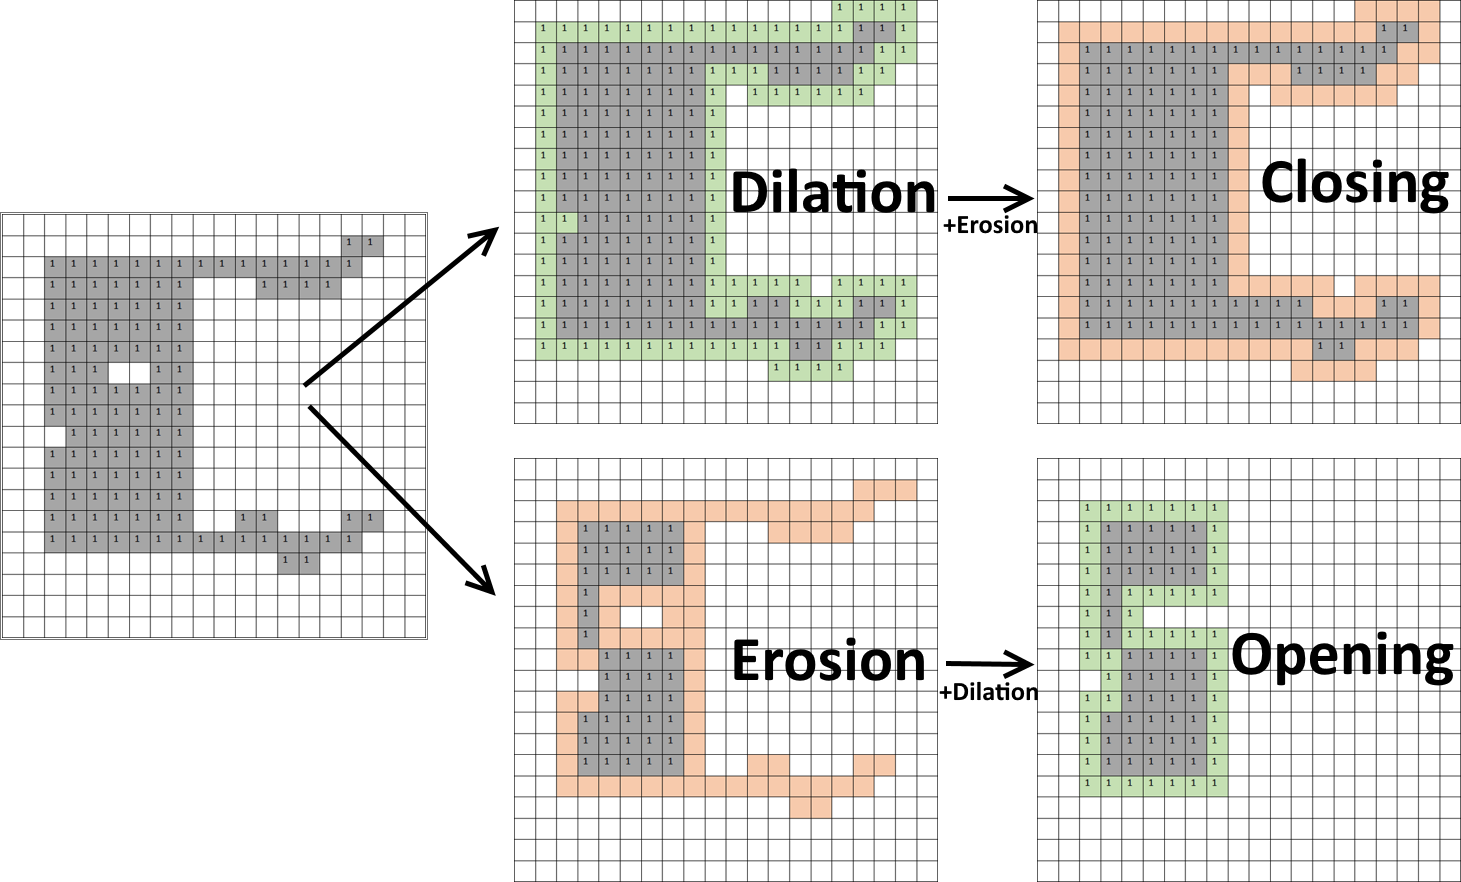
\includegraphics[width=1\textwidth]{media/morph/morph_all_text.png}
 \caption{Morphologische Operationen - Dilation, Erosion, Opening und Closing}
 \label{fig:boxfilter}
\end{figure}
